\subsubsection{\emph{Performance Measures} (PM)}

Avant d'optimiser, nous définissons sur le réseau cyclable des mesures de performance (\emph{Performance Measures}, PM). Cela reprend l'objectif de recherche d'équité, détaillé dans la section \ref{sect:equite}. 

Le procédé est le suivant : nous définissons un PM pour chaque carreau, nous calculons le PM. Ensuite, nous optimisons le réseau cyclable. Enfin, nous mesurons de nouveau le PM sur le réseau cyclable amélioré. Ainsi, nous pouvons comparer l'amélioration du réseau cyclable sur des critères précis.

C'est l'observation de l'existant qui pousse à la création d'un PM, de sorte à le quantifier, et le PM lui même pousse à développer des critères d'optimisation.


% \textcolor{red}{revoir avec derniere partie de ce .tex}

% %---- 

\subsubsection{Critères retenus}


L'objectif est de faire un modèle d'aide à la décision pour la métropole de Tours, afin de trouver les meilleurs tronçons à aménager pour améliorer l'équité du réseau cyclable. Dans notre modélisation, "aménager" un tronçon se traduit par "mettre au minimum son niveau LTS".

Nous avons retenu 3 critères d'optimisation différents :

\begin{enumerate} \label{criteresopti}
    \item le nombre de POI totaux atteints par les carreaux, \label{criterepoi}
    \item la population pouvant atteindre un POI, \label{criterepopu}
    \item le nombre de catégories différentes de POI atteintes par chaque carreau. \label{criterecat}
\end{enumerate}

La problématique de l'optimisation est la suivante : en se donnant une distance maximale \verb|dmax| entre un noeud délégué et un POI, un niveau LTS maximal pour les tronçons que nous pouvons emprunter et un budget à ne pas dépasser (en mètres), trouver les meilleurs tronçons à aménager.

\subsubsection{Modèles exacts} \label{modelesexacts}

Une manière d'optimiser le réseau cyclable est d'utiliser la programmation linéaire en nombres entiers (PLNE), en variables de décision binaires. 

Pour construire le modèle, nous faisons tout d'abord l'hypothèse suivante : le coût d'une amélioration est proportionnel à la distance de l'arc modifié, le budget peut donc s'exprimer en mètres de route à aménager.

% Les paramètres du modèle sont les suivants :

% Pour représenter le réseau cyclable (c'est à dire toutes les routes et chemins pouvant être empruntés potentiellement par les cyclistes), nous utilisons un graphe orienté $G(X, A)$ avec $X \ ( \vert X \vert = n)$ l'ensemble des nœuds et $A$ l'ensemble des arcs. A chaque arc est associé son coût en distance, et son danger. 



% On dispose également de l'ensemble des carreaux Filosofi couvrant le graphe, appelé $Z$. Nous conservons les carreaux dont la population n'est pas nulle.

% Pour chaque carreau, on trouve le nœud $n_z$ $\in$ $X$ le plus proche du centre. Pour chaque carreau $z$, on dispose d'une liste de POI potentiels, notés $L_z$, représentant les POI potentiellement accessibles depuis $n_z$ en $dmax$ km si l'ensemble du réseau était amélioré, c'est-à-dire si toutes les routes étaient sécurisées. Enfin, la fonction succ($i$) renvoie les successeurs du nœud $i$ dans le graphe $G$, et la fonction pred($i$) renvoie les prédécesseurs du nœud $i$ dans le graphe $G$.


%-----------

Les critères d'optimisation listés en \ref{criteresopti} se traduisent en :

\begin{enumerate}
    \item Minimiser la somme sur tous les carreaux du nombre de POI qui lui sont potentiellement accessibles en moins de \texttt{dmax}, mais qui ne sont pas atteints à cause du danger des voies,
    \item Minimiser la somme sur tous les carreaux du nombre de POI qui lui sont potentiellement accessibles en moins de \texttt{dmax}, mais qui ne sont pas atteints à cause du danger des voies, \textbf{multiplié} par la population de ce carreau,
    \item Maximiser la somme sur tous les carreaux du nombre de catégories de POI atteintes par le carreau parmi celles qui lui sont potentiellement accessibles.
\end{enumerate}

Les POI potentiellement accessibles (PPOI, \emph{Potential POI}) sont les POI qu'il serait possible d'atteindre si le niveau LTS de chaque tronçon de route était assez faible pour que l'on s'autorise à passer dessus, dans la limite de distance \texttt{dmax}. Ils sont toujours potentiellement accessibles par rapport à un carreau, un POI peut être potentiellement accessible pour un carreau mais trop loin pour un autre carreau.Les POI potentiellement accessibles mais non atteints sont donc les POI dans cette catégorie, mais qui se sont pas atteints avec les niveaux LTS réels sur chaque tronçon. 

Nous avons donc les fonctions objectives :

\begin{enumerate} \label{enum:function_obj}
    \item $\Minimize \sum_{z \in \mathcal{Z} } \sum_{p \in \mathcal{L}_z} \overline{PPOI_z^p}$,
    \item $\Minimize \sum_{z \in \mathcal{Z} } \sum_{p \in \mathcal{L}_z} \overline{PPOI_z^p} \times w_z$,
    \item $\Maximize \sum_{z \in \mathcal{Z} } \sum_{c \in \mathcal{C}} cat_c^z$.
\end{enumerate}

Avec :

\begin{itemize}
    \item $Z$ : ensemble des carreaux,
    \item $\mathcal{L}_z$ : visibilité du carreau $z$,
    \item $\overline{PPOI_z^p}=
    \begin{cases}
        1 \text{ si le POI $p$ (potentiellement accessible par $z$) n'est pas atteint,} \\
        0 \text{ sinon,}
    \end{cases}$
    \item $\mathcal{C}$ : ensemble des catégories,
    \item $cat_c^z=
    \begin{cases}
        1 \text{ si la catégorie $c$ est atteinte par le carreau $z$,} \\
        0 \text{ sinon,}
    \end{cases}$
    \item $w_z$ : population du carreau $z$.
\end{itemize}

On ajoute en plus des variables modélisant les arcs, indiquant si un arc est aménagé ou non, si un arc appartient au chemin entre le carreau $z$ et le POI $p$..., ainsi que des contraintes imposant la distance maximale d'un chemin carreau-POI, le budget à ne pas dépasser, la consistance d'un chemin...

Les modèles complets se trouvent en annexe.

\subsubsection{Heuristiques}\label{sect:heuristiquesopt}

Le gros de mon travail lors de ce stage a été de développer des heuristiques cherchant à optimiser l'équité d'un réseau cyclable, d'une manière similaire aux modèles exacts. 

L'intérêt de développer des heuristiques, c'est de pouvoir trouver des solutions rapidement, même si elles ne sont pas optimales. En effet, les modèles exacts prennent souvent trop de temps pour être utilisables, en particulier lorsqu'on travaille avec d'autres acteurs. Dans notre cas, le modèle exact que j'ai récupéré au début de mon stage était utilisable seulement pour une distance \verb|dmax| de 500 mètres sur le graphe représeentant la ville de Tours, alors qu'on aimerait avoir des résultats pour \verb|dmax| = 5 km.

En plus de l'aspect temporel, les modèles exacts demandent beaucoup de ressources et de mémoire, ce qui soulève des problèmes pratiques et écologiques. 

Les heuristiques que j'ai développées sont basées sur l'idée suivante : améliorer les plus courts chemins (PCC) partant d'un carreau et arrivant à un POI accessible par le carreau. L'hypothèse derrière cela est qu'un bon chemin à améliorer entre un carreau et un POI est souvent le PCC, en particulier pour les POI se trouvant proches d'un carreau.

Pour les heuristiques sur la population et sur le nombre de POI, nous utilisons l'algorithme \ref{hpcc}.  

\begin{algorithm}[!ht]
\DontPrintSemicolon
\caption{Heuristique PCC}
\label{hpcc}
\Donnees{graphe, carreaux, dmax, lts\_max, budget}
\Res{Choix de certains arcs à aménager}
\emph{calculer} les PCC et les stocker dans le vecteur pccs\;
\emph{trier}(pccs) \Comment*[l]{différentes manières de trier le vecteur}
\TantQue{pccs non vide}{
    pcc $\leftarrow$ dernier élément de pccs\;
    supprimer le dernier élément de pccs\;
    \PourCh{arc e dans pcc}{
        \Si{budget $\ge$ e.coût \textbf{et} e.amélioré=faux \textbf{et} e.lts $>$ lts\_max}{
            budget $\leftarrow$ budget - e.coût\;
            e.amélioré $\leftarrow$ vrai\;
        }
    }
}
\end{algorithm}

Plusieurs tris sur le vecteur \texttt{pccs} ont été testés : 
\begin{itemize} \label{item:tris}
    \item trier \texttt{pccs} dans l'ordre décroissant de la distance restante à aménager (\verb|hdist|). Le PCC ayant la distance à aménager la plus courte est donc choisi en premier.
    \item trier \texttt{pccs} dans l'ordre croissant de la population du carreau de départ du PCC (\verb|hpop|). Les PCC partant du carreau ayant le plus d'habitants sont alors choisis en premier.
    \item trier \texttt{pccs} dans l'ordre décroissant du ratio $\fFrac{\text{distance à aménager}}{\text{population du carreau}}$ (\verb|hpopdist|).
\end{itemize}


Une heuristique où l'on s'arrêtait prématurément, sans utiliser tout le budget, (algorithme \ref{hpcc2}) a aussi été testée. 

\begin{algorithm}[!ht]
\DontPrintSemicolon
\caption{Heuristique PCC sans utiliser tout le budget}
\label{hpcc2}
\Donnees{graphe, carreaux, dmax, lts\_max, budget}
\Res{Choix de certains arcs à aménager}
\emph{calculer} les PCC et les stocker dans le vecteur pccs\;
\emph{trier}(pccs) 
added\_edges $\leftarrow$ vecteur vide \;
\TantQue{budget $>$ 0 \textbf{et} pccs non vide}{
    pcc $\leftarrow$ dernier élément de pccs\;
    added\_complete\_pcc $\leftarrow$ vrai\;
    \PourCh{arc e dans pcc}{
        \Si{budget $>$ 0}{
            \Si{e.amélioré = faux \textbf{et} e.lts $>$ lts\_max}{
                budget $\leftarrow$ budget - e.coût\;
                e.amélioré $\leftarrow$ vrai\;
                ajouter e à added\_edges\;
            }
        }
        \Comment*[l]{si l'on dépasse le budget, on retire la dernière arête ajoutée}
        \Si{budget $<$ 0}{
            e $\leftarrow$ dernier élément de added\_edges\;
            e.amélioré $\leftarrow$ faux\;
            retirer e de added\_edges\;
            budget $\leftarrow$ budget + e.coût\;
            added\_complete\_pcc $\leftarrow$ faux\;
            \textbf{break}\;
        }
    }
    \Si{added\_complete\_pcc = vrai}{
        supprimer le dernier élément de pccs\;
    }
    \Sinon{
        \textbf{break} \Comment*[l]{on arrête dès qu'on ne peut plus aménager un arc}
    }
}
\end{algorithm}

Pour l'optimisation sur le nombre distinct de catégories atteintes par chaque carreau, nous utilisons l'algorithme \ref{hpccdiv}. Cet algorithme est similaire à l'algorithme \ref{hpcc}, mais il trie les PCC en fonction du nombre de catégories atteintes par le carreau de départ du PCC. L'idée est de maximiser le nombre de catégories atteintes par les carreaux, tout en s'occupant en priorité des carreaux qui atteignent le moins de catégories, dans un objectif d'équité.

Cet aspect d'équité n'est pas pris en compte dans le modèle exact associé, qui va lui maximiser le nombre de catégories atteintes par les carreaux, indépendamment du nombre de catégories déjà atteintes par les carreaux.

\begin{algorithm}[!ht]
\DontPrintSemicolon
\caption{Heuristique diversité de catégories}
\label{hpccdiv}
\Donnees{graphe, carreaux, dmax, lts\_max, budget}
\Res{Choix de certains arcs à aménager}
\emph{calculer} les PCC et les stocker dans le vecteur pccs\;
pccs $\leftarrow$ $\forall$ carreau, $\forall$ catégorie, conserver seulement le PCC reliant le carreau au POI de la catégorie auquel il reste le moins à aménager (si le PCC existe)\;
\emph{trier\_par\_diversité\_décroissante}(pccs) \Comment*[l]{trier les pcc en fonction du nombre de catégories qu'atteignent leur carreau de départ} %, dans un objectif d'équité
\TantQue{pccs non vide}{
    pcc $\leftarrow$ dernier élément de pccs\;
    supprimer le dernier élément de pccs\;
    \PourCh{arc e dans pcc}{
        \Si{budget $\ge$ e.coût \textbf{et} e.amélioré=faux \textbf{et} e.lts $>$ lts\_max}{
            budget $\leftarrow$ budget - e.coût\;
            e.amélioré $\leftarrow$ vrai\;
        }
    }
    \Si{le pcc est aménagé entièrement \textbf{et} que sa distance à aménager était non nulle}{
        nombre\_de\_catégories\_atteintes(pcc.carreau)+=1\;
        \emph{trier\_par\_diversité\_décroissante}(pccs) \Comment*[l]{repositionner correctement les PCC du carreau pour lequel on vient d'atteindre une nouvelle catégorie}
    }
}
\end{algorithm}

Il faut garder en tête que modifier le nombre de catégories atteintes par un carreau lorsqu'on aménage entièrement un PCC (dont la distance à aménager n'est pas nulle) n'est pas exactement recalculer le nombre de catégories qu'atteingnent tous les carreaux. En effet, une ou plusieurs des arêtes de ce PCC pourraient permettre aussi à un autre carreau d'atteindre une nouvelle catégorie, par effet de bord. Mais cela permet de gagner considérablement en vitesse.

Le calcul des PCC, étape commune à toutes les heuristiques, se fait en utilisant le graphe, les carreaux, la distance maximale ainsi que le facteur lts\_max (algorithme \ref{algo:dij}). Pour chaque carreau, nous appliquons un algorithme de Dijkstra à son noeud délégué et au graphe entier. Pour chaque noeud, nous stockons en plus de son prédecesseur la distance à aménager pour arriver jusqu'à ce noeud (nous stockons la distance à aménager, mais les PCC sont les PCC au sens de la distance totale, et non pas juste la distance à aménager). En ayant stocké ces informations, nous construisons ensuite les PCC selon l'algorithme \ref{algo:const_pcc}.

Cela s'effectue en même temps que le calcul des arcs et noeuds se trouvant dans la visibilité PCC des carreaux, pour économiser du temps de calcul. 


\begin{algorithm}[!ht]
\DontPrintSemicolon
\caption{Initialisation de la visibilité PCC}
\label{algo:dij}
\Donnees{graphe, carreaux, dmax, lts\_max}
\Res{Stockage des arcs et noeuds dans la visibilité de chaque carreau, ainsi que des prédecesseurs et distances à aménager}
\PourCh{carreau}{
    carreau.predecesseurs\_et\_distance\_à\_aménager $\leftarrow$ map vide\;

    \textit{S} $\leftarrow$ pile vide de nœuds\;
    \textit{R} $\leftarrow$ pile vide de de nœuds à reset\;
    \emph{initialiser tous les nœuds :} distance = $\infty$, distance\_à\_aménager = $\infty$, visité = faux \;
    \textit{u} $\leftarrow$ nœud central du carreau\;u.distance $\leftarrow 0$, u.distance\_à\_aménager $\leftarrow 0$, u.visité $\leftarrow$ vrai\;
    \emph{empiler} u dans \textit{S} et \textit{R}\;
    \TantQue{\textit{S} non vide}{
        v $\leftarrow$ noeud de \textit{S} tel que v.distance soit minimal \;
        \emph{ajouter} v à la visibilité du carreau \Comment*[l]{visibilité en terme de noeuds}
        \PourCh{arc \textit{e} sortant de v}{
            w $\leftarrow$ autre extrémité de \textit{e}\;
            % \Comment*[l]{calcul des nouvelles étiquettes}\;
            nouvelle\_distance $\leftarrow$ v.distance + e.coût \Comment*[l]{le cout étant la longueur d'un arc}
            nouvelle\_distance\_à\_aménager $\leftarrow$ v.distance\_à\_aménager\;

            \Comment*[l]{s'il faut aménager cet arc pour qu'il soit utilisable, on met à jour la distance à aménager}
            \Si{e.LTS > lts\_max}{
                nouvelle\_distance\_à\_aménager $\leftarrow$ nouvelle\_distance\_à\_aménager + e.coût \;
            }
            \Si{nouvelle\_distance $\leq$ dmax \textbf{et} nouvelle\_distance $<$ w.distance}{
                % mise à jour
                w.distance $\leftarrow$ nouvelle\_distance\;
                w.distance\_à\_aménager $\leftarrow$ nouvelle\_distance\_à\_aménager\;
                \Si{w.visité = faux}{
                    w.visité $\leftarrow$ vrai\;
                    empiler w dans \textit{S} et \textit{R}\;
                }
                % ajouter l'arête visible
                \emph{ajouter} e à la visibilité du carreau \Comment*[l]{visibilité en terme d'arcs}
                % stocker prédécesseur et distance à aménager
                carreau.predecesseurs\_et\_distance\_à\_aménager[w.id] $\leftarrow$ (v, nouvelle\_distance\_à\_aménager) \Comment*[l]{c'est une map, donc les informations sur w sont modifiables}
            }
        }
    }
    \Comment*[l]{Nous enregistrons quels noeuds et arcs sont dans la visibilité du carreau, et quels noeuds permettent de rencontruiste les PCC du carreau, ainsi que leur distances à aménager. On peut alors réitialiser les noeuds et passer au prochain carreau.}
}
\end{algorithm}

\begin{algorithm}[!ht]
\DontPrintSemicolon
\caption{Construction des PCC}
\label{algo:const_pcc}
\Donnees{graphe, carreaux}
\Res{Liste des PCC}
pccs $\leftarrow$ liste vide \;
\PourCh{carreau}{
    \PourCh{POI potentiellement accessible par le carreau $p$}{
        \Si{$p$ $\neq$ noeud central du carreau}{
            chemin $\leftarrow$ liste vide\;
            here $\leftarrow p$ \;
            pred, dist $\leftarrow$ prédécesseur et distance à aménager pour here\;
            \TantQue{pred $\neq$ nul}{
                \emph{insérer} l'arête (pred, here) au début de chemin\;
                here $\leftarrow$ pred\;
                pred, dist $\leftarrow$ prédécesseur et distance à aménager pour here\;
            }
            pcc $\leftarrow$ un nouveau PCC avec les informations (carreau d'origine, $p$, distance à aménager, chemin, population)\;
            \emph{ajouter} pcc à pccs\;
        }
    }
}
\end{algorithm}

\subsubsection{Deux visibilités différentes} \label{sect:2visi}

L'optimisation par CPLEX s'effectue sur deux visibilités différentes : 

\begin{itemize}
    \item La \textbf{visibilité exacte}, où la visibilité d'un carreau comprend tous les arcs qui lui sont à une distance inférieure à la distance maximale \texttt{dmax}. Etant donné que \texttt{dmax} ne peut pas être dépassé lors de la recherche du résultat optimal, ce modèle donne le même résultat que si tout le graphe était visible, la visibilité est bien exacte. Cette technique permet de rendre CPLEX plus rapide, parce qu'on ne créé pas de variables correspondant aux couples carreaux-POI et pour les triplets carreaux-POI-arcs dans un chemin impossibles.

    \item La \textbf{visibilité PCC/visibilité réduite}, où la visibilité d'un carreau comprend toutes les arêtes qui sont dans un PCC d'un nœud délégué jusqu'à un point d'intérêt, tout en respectant la contrainte de distance de la visibilité précédente. La visibilité d'un carreau comprend aussi les arêtes se trouvant dans un PCC allant d'un nœud délégué d'un \emph{autre} carreau à un POI, tant que ces arêtes sont à moins de \texttt{dmax} de distance du carreau. Voir figure \ref{fig:smallvisi}.
\end{itemize} 

\begin{figure}[!ht]
    \centering
    \begin{subfigure}[t]{0.3\textwidth}
        \centering
        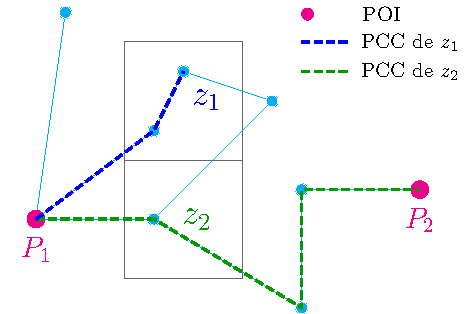
\includegraphics[width=0.92\linewidth]{PDFs/graph.pdf}
    \caption{Considérons un graphe avec 2 POI. Supposons que, en une distance \texttt{dmax}, $P_1$ soit accessible à la fois par $z_1$ et $z_2$, un PCC existe donc de $z_1$ à $P_1$ et de $z_2$ à $P_1$. Supposons aussi que $P_2$ ne soit accessible que par $z_2$. Un PCC existe de $z_2$ à $P_2$, mais pas de $z_1$ à $P_2$. }
    \end{subfigure}
    \hfill
    \begin{subfigure}[t]{0.3\textwidth}
        \centering
        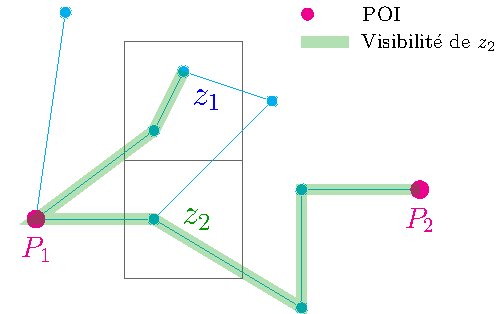
\includegraphics[width=1\linewidth]{PDFs/visi_z2.pdf}
    \caption{Si l'on suppose qu'en passant seulement par un arc hachuré en vert ou bleu, en moins de \texttt{dmax} il est possible d'aller de $z_2$ jusqu'à $z_1$, la visibilité de $z_2$ est celle ci dessus.}
    \end{subfigure}
    \hfill
    \begin{subfigure}[t]{0.3\textwidth}
        \centering
        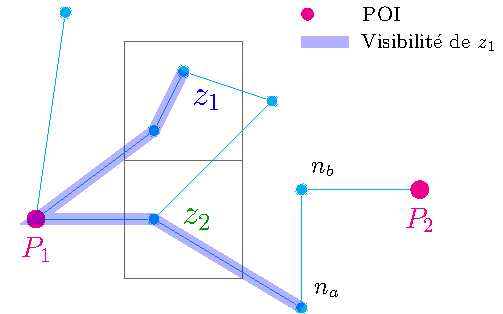
\includegraphics[width=1\linewidth]{PDFs/visi_z1.pdf}
    \caption{Si l'on suppose qu'en passant seulement par un arc hachuré en vert ou bleu, en moins de \texttt{dmax} il est possible d'aller de $z_1$ jusqu'à $n_a$, mais pas jusqu'à $n_b$, la visibilité de $z_1$ est celle ci dessus.}
    \end{subfigure}
    \caption{Visibilité PCC}
    \label{fig:smallvisi}
\end{figure}

Les noeuds visibles sont ceux qui appartiennent à un arc dans la visibilité.

La visibilité pour les heuristiques est toujours la seconde. L'intérêt de faire un modèle exact sur la seconde visibilité est d'avoir un modèle plus rapide que le modèle exact sur la visibilité exacte, mais aussi de pouvoir comparer les performances des heuristiques. Il existe donc deux modèles exacts :
\begin{itemize}
    \item un modèle exact sur la visibilité exacte,
    \item un modèle exact sur la visibilité PCC.
\end{itemize}

On remarque que procéder comme dans l'algorithme \ref{algo:dij} ne donne pas exactement la visibilité PCC, puisqu'on ajoute des arcs et arêtes qui ne sont pas dans un PCC noeud délégué-POI. Il faut ensuite supprimer les arcs et noeuds de la visibilité qui ne sont pas dans les PCC, c'est à dire parcourir encore une fois tous les carreaux (ce que je fais dans une fonction différente de la fonction codant l'algorithme \ref{algo:dij}). Il aurait peut être été pertinent d'organiser les étapes différemment, pour économiser du temps de calcul, mais cela aurait été plus compliqué à mettre en place.

La valeur objective des modèles exacts dépend aussi de la visibilité sur laquelle on la calcule. Cela est davantage détaillé en section \ref{sect:prog_modelesexacts}.


\subsubsection{Pertinence des résultats trouvés}

Les modèles utilisés sont incomplets par rapport à la réalité du terrain. Ils ne se soucient pas, par exemple, d'à quel point il est facile d'aménager tel ou tel tronçon. De plus, l'hypothèse sur le budget est simpliste. En réalité, le budget alloué à l'aménagement des tronçons peut varier en fonction de nombreux facteurs, tels que la complexité des travaux, les contraintes techniques, ou encore les enjeux environnementaux. Les modèles ne prennent pas non plus en compte les effets à long terme des aménagements proposés. Par conséquent, les résultats obtenus doivent être interprétés avec prudence et complétés par des études de terrain et des consultations avec les acteurs locaux.

C'est l'intérêt de travailler avec des cartographes, qui connaissent la réalité du terrain et ces problématiques.